\documentclass[a4paper,12pt]{article}
\usepackage[utf8]{inputenc}
\usepackage{float}
\usepackage{listings}
\usepackage[margin=1in]{geometry}
\setlength\parindent{0pt}
\usepackage{xcolor}
\usepackage{graphicx}
\definecolor{dkgreen}{rgb}{0,0.6,0}
\definecolor{dred}{rgb}{0.545,0,0}
\definecolor{dblue}{rgb}{0,0,0.545}
\definecolor{lgrey}{rgb}{0.9,0.9,0.9}
\definecolor{gray}{rgb}{0.4,0.4,0.4}
\definecolor{darkblue}{rgb}{0.0,0.0,0.6}
\renewcommand\floatpagefraction{0.8} %% default value: 0.5
\renewcommand\topfraction{0.8} 
\lstdefinelanguage{cpp}{
      backgroundcolor=\color{lgrey},  
      basicstyle=\footnotesize \ttfamily \color{black} \bfseries,   
      breakatwhitespace=false,       
      breaklines=true,               
      captionpos=b,                   
      commentstyle=\color{dkgreen},   
      deletekeywords={...},          
      escapeinside={\%*}{*)},                  
      frame=single,                  
      language=C++,                
      keywordstyle=\color{purple},  
      morekeywords={BRIEFDescriptorConfig,string,TiXmlNode,DetectorDescriptorConfigContainer,istringstream,cerr,exit}, 
      identifierstyle=\color{black},
      stringstyle=\color{blue},      
      numbers=right,                 
      numbersep=5pt,                  
      numberstyle=\tiny\color{black}, 
      rulecolor=\color{black},        
      showspaces=false,               
      showstringspaces=false,        
      showtabs=false,                
      stepnumber=1,                   
      tabsize=5,                     
      title=\lstname,                 
    }

\begin{document}
%opening
\title{CS352 HW1 Design Principles}
\author{Jason Dorweiler}
\maketitle 

For this assignment I will critique the design principles used in the Widows version of the Spotify app. \\

\textbf{Visibility}

The buttons that a user is most likely to quickly need are very visible.  Some examples of this are in the lower left where the buttons to skip, play, and pause songs are clearly visible.  There are also the same controls on the center of the screen near the album covers.  

Other than the song control buttons everything else seems to violate visibility.  The whole page is too cluttered and there is just way too much going on in one page.  I think it would make it difficult for a new user to find any of the other controls that they're looking for. \\

\begin{figure}[h!]
\centering
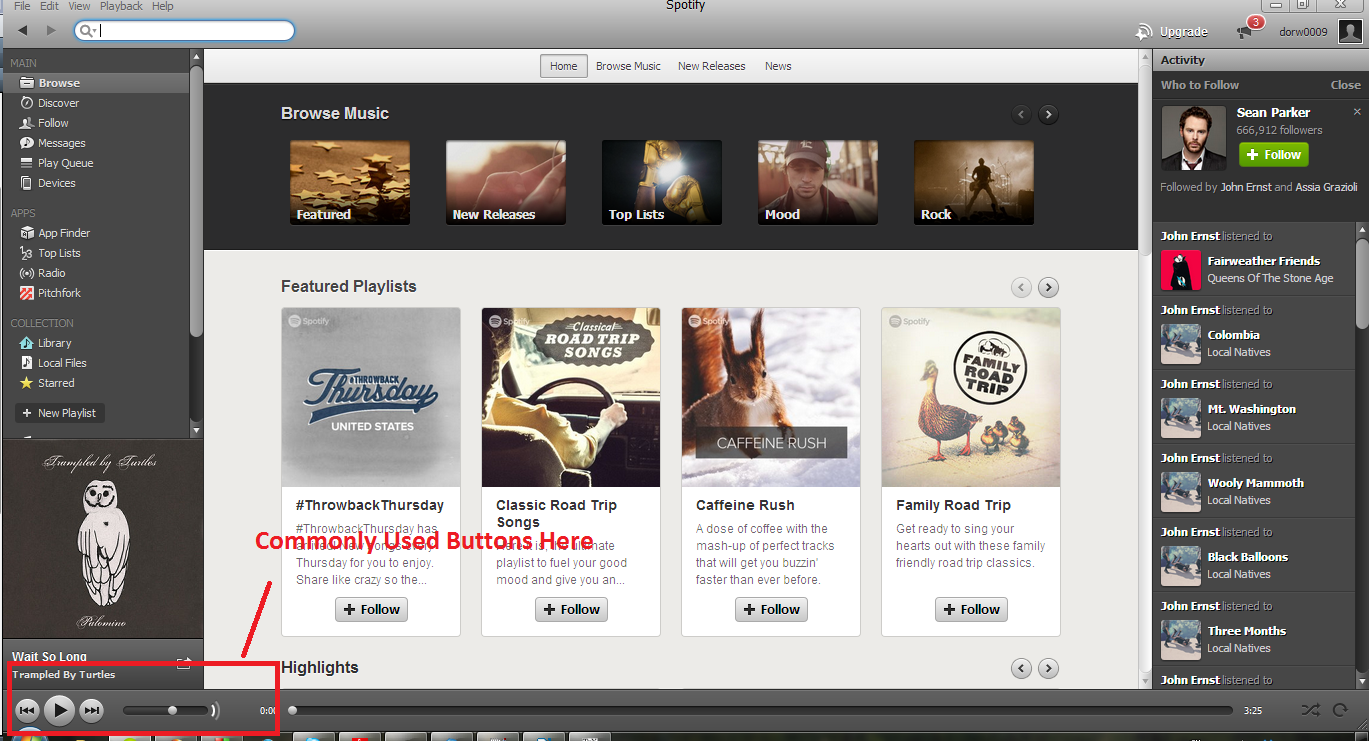
\includegraphics[width=1\textwidth]{visibility}
\caption{Showing easily visible controls}
\end{figure}


\textbf{Feedback}

All of the buttons and menus in this app have some way of providing feedback.  Some of the buttons that need to be clicked will highlight when you hover over them and then visually depress when clicked.  Other menu items such as the Main, Apps, and Collection menus on the left will highlight when clicked. 

It was hard to find anything on  the app that violates the feedback principle.  One small thing is that the left menu doesn't highlight when you hover over it.  In the picture I've shown that happens after the menu item is clicked.  I think that would be a good feedback addition.

\begin{figure}[h!]
\centering
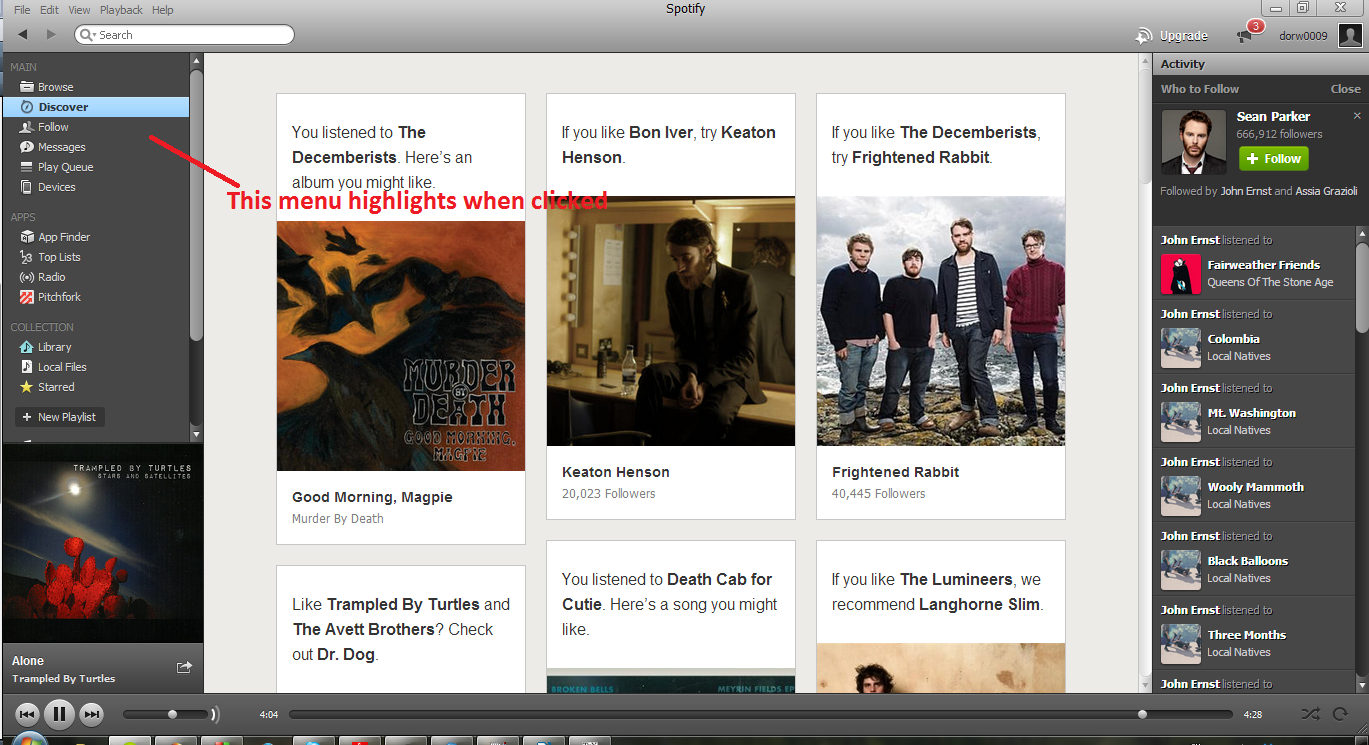
\includegraphics[width=1\textwidth]{feedback}
\caption{Showing feedback menu highlighting}
\end{figure}

\textbf{Constraint}

The app uses constraints on the user drop down menu on the top right.  This menu limits the user to only picking from a specific number of options.  There is also a top bar menu which only allows the user to pick from a list of predetermined options.  There are really no options for the user to do anything that the designers didn't intend.

One thing I found is in the search bar on the top there is still a chance that the user could make a typo in their search term.  They seem to have tried to minimize that by having a window appear under the search as you type.  This window try to guess what you are searching for and fixes typos.  But that still wont stop a user from making them.

\begin{figure}[H]
\centering
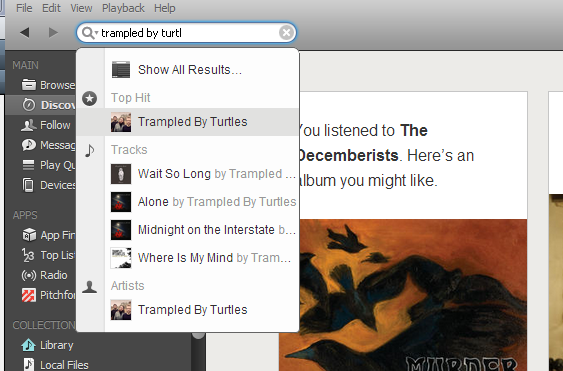
\includegraphics[width=0.6\textwidth]{constraint}
\caption{The search box uses constraint by trying to predict a users search.  This can help prevent typo erros}
\end{figure}


\textbf{Consistency}


The consistency of the whole app seems very good and I had a hard time trying to find something that didn't fit.  Some of the consistency things I found: everything is done by left clicking, and menu items on the top bar group similar operations together.    
One consistency problem I found was in the play, rewind, and fast forward buttons.  They all use the same symbols and have the same function. But they vary in size and color at different areas throughout the program.  To be consistent they should have the same buttons throughout.  Another consistency problem I found is in the vertical window sliders (green boxes).  There are three of them.  One on the left menu, one for the big main window in the middle, and a smaller on on the right.  The left and right sliders have the same color but the middle one is a different color.  

\begin{figure}[H]
\centering
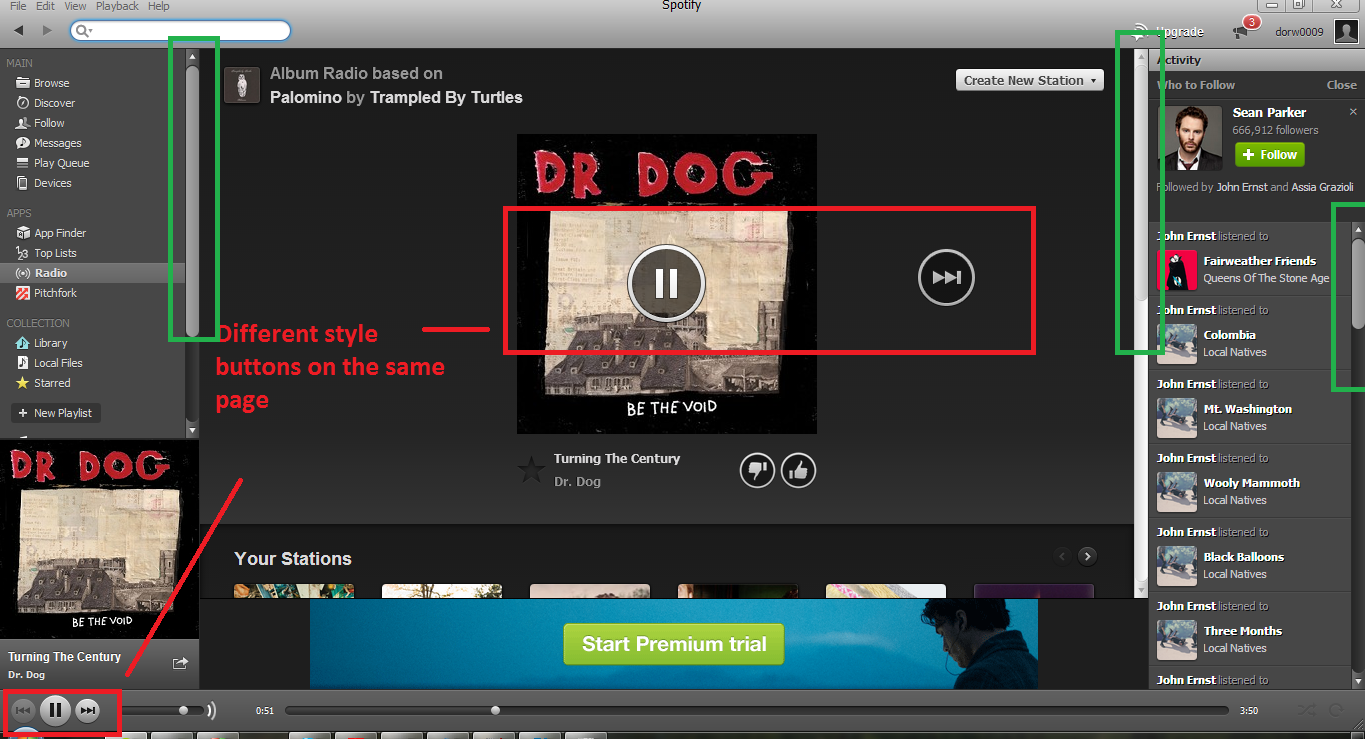
\includegraphics[width=1\textwidth]{consistency}
\caption{Different colored sliders}
\end{figure}
\newpage
\textbf{Affordance}

There are a lot of buttons in this which lead you to want to click them.  Some examples are in the song controls (play, rewind, etc...) and in the button used to create new stations.  These buttons are obviously intended to be clicked.  The song's volume and position sliders use a design which tells you that you should click and drag them. 

There are a few things that seem to violate the affordance design principle.  Several of the buttons don't even look like buttons and so without actually trying a user wouldn't know if they should be clicked or not.  I circled some of these buttons in the image.  

\begin{figure}[H]
\centering
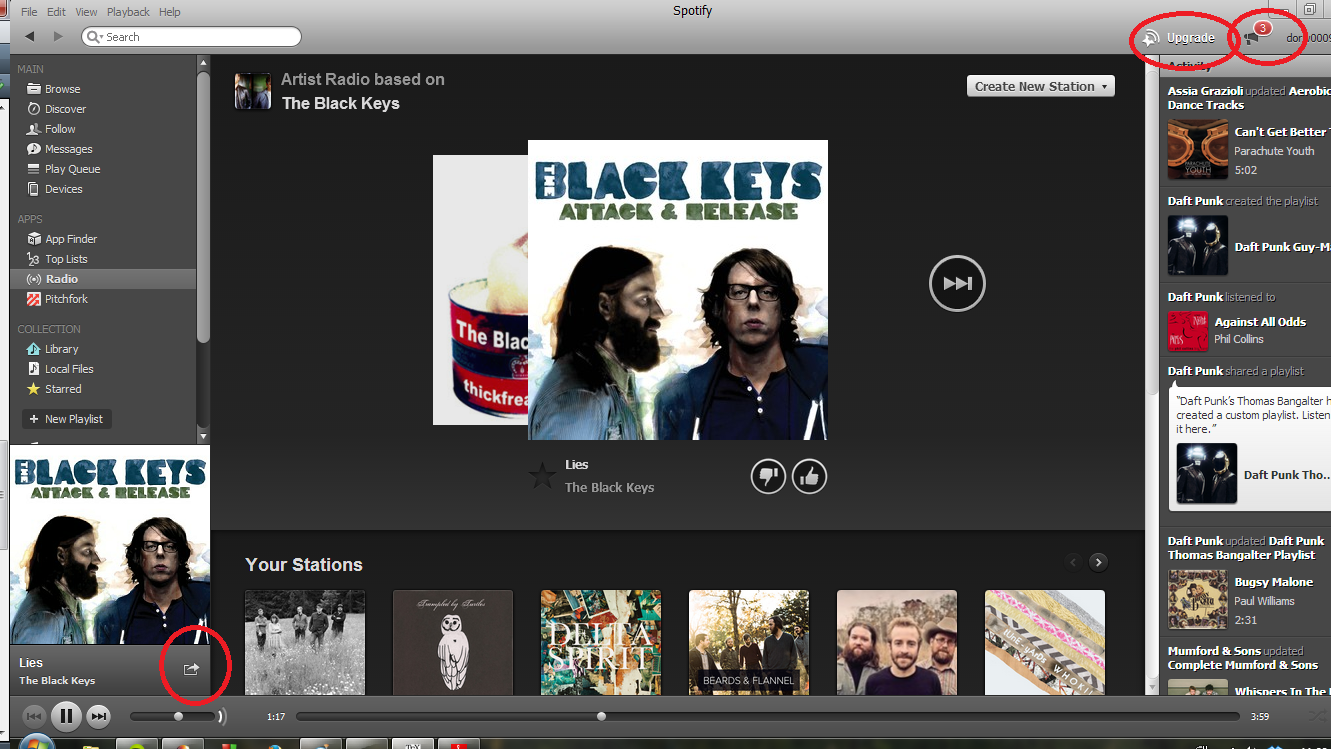
\includegraphics[width=1\textwidth]{affordance}
\caption{Some buttons that violate the affordance design principle circled in red}
\end{figure}

\end{document}